\documentclass[twoside]{book}

% Packages required by doxygen
\usepackage{fixltx2e}
\usepackage{calc}
\usepackage{doxygen}
\usepackage[export]{adjustbox} % also loads graphicx
\usepackage{graphicx}
\usepackage[utf8]{inputenc}
\usepackage{makeidx}
\usepackage{multicol}
\usepackage{multirow}
\PassOptionsToPackage{warn}{textcomp}
\usepackage{textcomp}
\usepackage[nointegrals]{wasysym}
\usepackage[table]{xcolor}

% Font selection
\usepackage[T1]{fontenc}
\usepackage[scaled=.90]{helvet}
\usepackage{courier}
\usepackage{amssymb}
\usepackage{sectsty}
\renewcommand{\familydefault}{\sfdefault}
\allsectionsfont{%
  \fontseries{bc}\selectfont%
  \color{darkgray}%
}
\renewcommand{\DoxyLabelFont}{%
  \fontseries{bc}\selectfont%
  \color{darkgray}%
}
\newcommand{\+}{\discretionary{\mbox{\scriptsize$\hookleftarrow$}}{}{}}

% Page & text layout
\usepackage{geometry}
\geometry{%
  a4paper,%
  top=2.5cm,%
  bottom=2.5cm,%
  left=2.5cm,%
  right=2.5cm%
}
\tolerance=750
\hfuzz=15pt
\hbadness=750
\setlength{\emergencystretch}{15pt}
\setlength{\parindent}{0cm}
\setlength{\parskip}{3ex plus 2ex minus 2ex}
\makeatletter
\renewcommand{\paragraph}{%
  \@startsection{paragraph}{4}{0ex}{-1.0ex}{1.0ex}{%
    \normalfont\normalsize\bfseries\SS@parafont%
  }%
}
\renewcommand{\subparagraph}{%
  \@startsection{subparagraph}{5}{0ex}{-1.0ex}{1.0ex}{%
    \normalfont\normalsize\bfseries\SS@subparafont%
  }%
}
\makeatother

% Headers & footers
\usepackage{fancyhdr}
\pagestyle{fancyplain}
\fancyhead[LE]{\fancyplain{}{\bfseries\thepage}}
\fancyhead[CE]{\fancyplain{}{}}
\fancyhead[RE]{\fancyplain{}{\bfseries\leftmark}}
\fancyhead[LO]{\fancyplain{}{\bfseries\rightmark}}
\fancyhead[CO]{\fancyplain{}{}}
\fancyhead[RO]{\fancyplain{}{\bfseries\thepage}}
\fancyfoot[LE]{\fancyplain{}{}}
\fancyfoot[CE]{\fancyplain{}{}}
\fancyfoot[RE]{\fancyplain{}{\bfseries\scriptsize Generated by Doxygen }}
\fancyfoot[LO]{\fancyplain{}{\bfseries\scriptsize Generated by Doxygen }}
\fancyfoot[CO]{\fancyplain{}{}}
\fancyfoot[RO]{\fancyplain{}{}}
\renewcommand{\footrulewidth}{0.4pt}
\renewcommand{\chaptermark}[1]{%
  \markboth{#1}{}%
}
\renewcommand{\sectionmark}[1]{%
  \markright{\thesection\ #1}%
}

% Indices & bibliography
\usepackage{natbib}
\usepackage[titles]{tocloft}
\setcounter{tocdepth}{3}
\setcounter{secnumdepth}{5}
\makeindex

% Hyperlinks (required, but should be loaded last)
\usepackage{ifpdf}
\ifpdf
  \usepackage[pdftex,pagebackref=true]{hyperref}
\else
  \usepackage[ps2pdf,pagebackref=true]{hyperref}
\fi
\hypersetup{%
  colorlinks=true,%
  linkcolor=blue,%
  citecolor=blue,%
  unicode%
}

% Custom commands
\newcommand{\clearemptydoublepage}{%
  \newpage{\pagestyle{empty}\cleardoublepage}%
}

\usepackage{caption}
\captionsetup{labelsep=space,justification=centering,font={bf},singlelinecheck=off,skip=4pt,position=top}

%===== C O N T E N T S =====

\begin{document}

% Titlepage & ToC
\hypersetup{pageanchor=false,
             bookmarksnumbered=true,
             pdfencoding=unicode
            }
\pagenumbering{roman}
\begin{titlepage}
\vspace*{7cm}
\begin{center}%
{\Large T\+P2\+\_\+a }\\
\vspace*{1cm}
{\large Generated by Doxygen 1.8.11}\\
\end{center}
\end{titlepage}
\clearemptydoublepage
\tableofcontents
\clearemptydoublepage
\pagenumbering{arabic}
\hypersetup{pageanchor=true}

%--- Begin generated contents ---
\chapter{Data Structure Index}
\section{Data Structures}
Here are the data structures with brief descriptions\+:\begin{DoxyCompactList}
\item\contentsline{section}{\hyperlink{structTLex}{T\+Lex} \\*Structure contenant tous les parametres/donnees pour l\textquotesingle{}analyse lexicale }{\pageref{structTLex}}{}
\item\contentsline{section}{\hyperlink{structTSymbole}{T\+Symbole} \\*Union permettant de manipuler un entier/reel/chaine pour la table des symboles }{\pageref{structTSymbole}}{}
\end{DoxyCompactList}

\chapter{File Index}
\section{File List}
Here is a list of all documented files with brief descriptions\+:\begin{DoxyCompactList}
\item\contentsline{section}{\hyperlink{paramcmdl_8c}{paramcmdl.\+c} \\*Contient le code des fonctions }{\pageref{paramcmdl_8c}}{}
\item\contentsline{section}{\hyperlink{paramcmdl_8h}{paramcmdl.\+h} \\*Contient les prototypes des fonctions }{\pageref{paramcmdl_8h}}{}
\item\contentsline{section}{\hyperlink{tp1__c_8c}{tp1\+\_\+c.\+c} \\*Contient la fonction main }{\pageref{tp1__c_8c}}{}
\end{DoxyCompactList}

\chapter{Data Structure Documentation}
\hypertarget{structTLex}{}\section{T\+Lex Struct Reference}
\label{structTLex}\index{T\+Lex@{T\+Lex}}


structure contenant tous les parametres/donnees pour l\textquotesingle{}analyse lexicale  




Collaboration diagram for T\+Lex\+:
% FIG 0
\subsection*{Data Fields}
\begin{DoxyCompactItemize}
\item 
char $\ast$ \hyperlink{structTLex_a2242e630c3f871659c3e36b101b504b4}{data}
\item 
char $\ast$ \hyperlink{structTLex_a1122e1ced17c2c07f7975b4f11110ad8}{start\+Pos}
\item 
int \hyperlink{structTLex_a74499b75b25dc1bce1fb2f66af6ce1e2}{nb\+Lignes}
\item 
\hyperlink{structTSymbole}{T\+Symbole} $\ast$ \hyperlink{structTLex_a31a6c4fc0839643e3251a372ba7adf04}{table\+Symboles}
\item 
int \hyperlink{structTLex_a84d0d3a30f4b42f8db675f8cbb60373f}{nb\+Symboles}
\end{DoxyCompactItemize}


\subsection{Detailed Description}
structure contenant tous les parametres/donnees pour l\textquotesingle{}analyse lexicale 

\subsection{Field Documentation}
\index{T\+Lex@{T\+Lex}!data@{data}}
\index{data@{data}!T\+Lex@{T\+Lex}}
\subsubsection[{\texorpdfstring{data}{data}}]{\setlength{\rightskip}{0pt plus 5cm}char$\ast$ T\+Lex\+::data}\hypertarget{structTLex_a2242e630c3f871659c3e36b101b504b4}{}\label{structTLex_a2242e630c3f871659c3e36b101b504b4}
chaine a parcourir \index{T\+Lex@{T\+Lex}!nb\+Lignes@{nb\+Lignes}}
\index{nb\+Lignes@{nb\+Lignes}!T\+Lex@{T\+Lex}}
\subsubsection[{\texorpdfstring{nb\+Lignes}{nbLignes}}]{\setlength{\rightskip}{0pt plus 5cm}int T\+Lex\+::nb\+Lignes}\hypertarget{structTLex_a74499b75b25dc1bce1fb2f66af6ce1e2}{}\label{structTLex_a74499b75b25dc1bce1fb2f66af6ce1e2}
nb de lignes analysees \index{T\+Lex@{T\+Lex}!nb\+Symboles@{nb\+Symboles}}
\index{nb\+Symboles@{nb\+Symboles}!T\+Lex@{T\+Lex}}
\subsubsection[{\texorpdfstring{nb\+Symboles}{nbSymboles}}]{\setlength{\rightskip}{0pt plus 5cm}int T\+Lex\+::nb\+Symboles}\hypertarget{structTLex_a84d0d3a30f4b42f8db675f8cbb60373f}{}\label{structTLex_a84d0d3a30f4b42f8db675f8cbb60373f}
taille du tableau table\+Symboles \index{T\+Lex@{T\+Lex}!start\+Pos@{start\+Pos}}
\index{start\+Pos@{start\+Pos}!T\+Lex@{T\+Lex}}
\subsubsection[{\texorpdfstring{start\+Pos}{startPos}}]{\setlength{\rightskip}{0pt plus 5cm}char$\ast$ T\+Lex\+::start\+Pos}\hypertarget{structTLex_a1122e1ced17c2c07f7975b4f11110ad8}{}\label{structTLex_a1122e1ced17c2c07f7975b4f11110ad8}
position de depart pour la prochaine analyse \index{T\+Lex@{T\+Lex}!table\+Symboles@{table\+Symboles}}
\index{table\+Symboles@{table\+Symboles}!T\+Lex@{T\+Lex}}
\subsubsection[{\texorpdfstring{table\+Symboles}{tableSymboles}}]{\setlength{\rightskip}{0pt plus 5cm}{\bf T\+Symbole}$\ast$ T\+Lex\+::table\+Symboles}\hypertarget{structTLex_a31a6c4fc0839643e3251a372ba7adf04}{}\label{structTLex_a31a6c4fc0839643e3251a372ba7adf04}
tableau des symboles \+: chaines/entier/reel 

The documentation for this struct was generated from the following file\+:\begin{DoxyCompactItemize}
\item 
\hyperlink{tp2__a_8c}{tp2\+\_\+a.\+c}\end{DoxyCompactItemize}

\hypertarget{structTSymbole}{}\section{T\+Symbole Union Reference}
\label{structTSymbole}\index{T\+Symbole@{T\+Symbole}}


union permettant de manipuler un entier/reel/chaine pour la table des symboles  


\subsection*{Data Fields}
\begin{DoxyCompactItemize}
\item 
int \hyperlink{structTSymbole_a3f1c09d456d42f56c7e97b767fcda611}{type}
\item 
\begin{tabbing}
xx\=xx\=xx\=xx\=xx\=xx\=xx\=xx\=xx\=\kill
union \{\\
\>int {\bfseries entier}\\
\>float {\bfseries reel}\\
\>char $\ast$ {\bfseries chaine}\\
\} \hyperlink{structTSymbole_a448dc40c2c8e5d050436fa598f528723}{val}\\

\end{tabbing}\end{DoxyCompactItemize}


\subsection{Detailed Description}
union permettant de manipuler un entier/reel/chaine pour la table des symboles 

\subsection{Field Documentation}
\index{T\+Symbole@{T\+Symbole}!type@{type}}
\index{type@{type}!T\+Symbole@{T\+Symbole}}
\subsubsection[{\texorpdfstring{type}{type}}]{\setlength{\rightskip}{0pt plus 5cm}int T\+Symbole\+::type}\hypertarget{structTSymbole_a3f1c09d456d42f56c7e97b767fcda611}{}\label{structTSymbole_a3f1c09d456d42f56c7e97b767fcda611}
l\textquotesingle{}un des 3 types suivants \+: J\+S\+O\+N\+\_\+\+S\+T\+R\+I\+N\+G/\+J\+S\+O\+N\+\_\+\+I\+N\+T\+\_\+\+N\+U\+M\+B\+E\+R/\+J\+S\+O\+N\+\_\+\+R\+E\+A\+L\+\_\+\+N\+U\+M\+B\+ER \index{T\+Symbole@{T\+Symbole}!val@{val}}
\index{val@{val}!T\+Symbole@{T\+Symbole}}
\subsubsection[{\texorpdfstring{val}{val}}]{\setlength{\rightskip}{0pt plus 5cm}union \{ ... \}   T\+Symbole\+::val}\hypertarget{structTSymbole_a448dc40c2c8e5d050436fa598f528723}{}\label{structTSymbole_a448dc40c2c8e5d050436fa598f528723}
valeur associer a un element de la table des symboles 

The documentation for this union was generated from the following file\+:\begin{DoxyCompactItemize}
\item 
\hyperlink{tp2__a_8c}{tp2\+\_\+a.\+c}\end{DoxyCompactItemize}

\chapter{File Documentation}
\hypertarget{tp2__a_8c}{}\section{tp2\+\_\+a.\+c File Reference}
\label{tp2__a_8c}\index{tp2\+\_\+a.\+c@{tp2\+\_\+a.\+c}}


analyseur lexical pour le langage J\+S\+ON  


{\ttfamily \#include $<$stdio.\+h$>$}\\*
{\ttfamily \#include $<$string.\+h$>$}\\*
{\ttfamily \#include $<$ctype.\+h$>$}\\*
{\ttfamily \#include $<$stdlib.\+h$>$}\\*
{\ttfamily \#include $<$assert.\+h$>$}\\*
Include dependency graph for tp2\+\_\+a.\+c\+:
\nopagebreak
\begin{figure}[H]
\begin{center}
\leavevmode
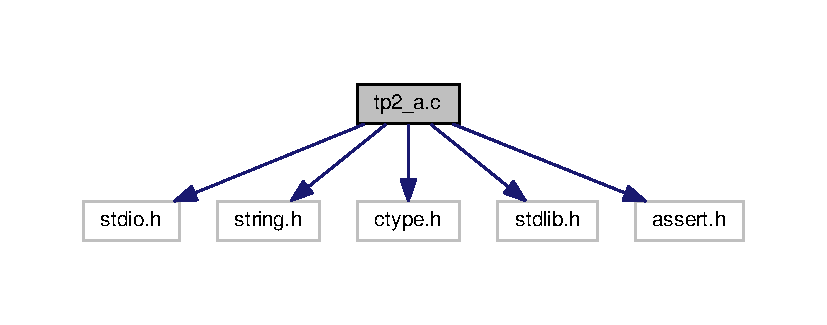
\includegraphics[width=350pt]{tp2__a_8c__incl}
\end{center}
\end{figure}
\subsection*{Data Structures}
\begin{DoxyCompactItemize}
\item 
union \hyperlink{structTSymbole}{T\+Symbole}
\begin{DoxyCompactList}\small\item\em union permettant de manipuler un entier/reel/chaine pour la table des symboles \end{DoxyCompactList}\item 
struct \hyperlink{structTLex}{T\+Lex}
\begin{DoxyCompactList}\small\item\em structure contenant tous les parametres/donnees pour l\textquotesingle{}analyse lexicale \end{DoxyCompactList}\end{DoxyCompactItemize}
\subsection*{Macros}
\begin{DoxyCompactItemize}
\item 
\#define \hyperlink{tp2__a_8c_a1c1d6b9a4119ed60f57af0732bbc7ac4}{J\+S\+O\+N\+\_\+\+L\+E\+X\+\_\+\+E\+R\+R\+OR}~-\/1
\item 
\#define \hyperlink{tp2__a_8c_a172a7e23fb0ac9f8ce19bee485090de7}{J\+S\+O\+N\+\_\+\+T\+R\+UE}~1
\item 
\#define \hyperlink{tp2__a_8c_a8944b24b93d4a397aa5748a5f6048d5b}{J\+S\+O\+N\+\_\+\+F\+A\+L\+SE}~2
\item 
\#define \hyperlink{tp2__a_8c_a47153ed2f7bd07cabffd495e4a18839f}{J\+S\+O\+N\+\_\+\+N\+U\+LL}~3
\item 
\#define \hyperlink{tp2__a_8c_a3b936ae16a984c94b371ed1e8bc74465}{J\+S\+O\+N\+\_\+\+L\+CB}~4
\item 
\#define \hyperlink{tp2__a_8c_a8505d4213a71673ca62aa1e799e4333c}{J\+S\+O\+N\+\_\+\+R\+CB}~5
\item 
\#define \hyperlink{tp2__a_8c_afc6172b33cb8b8fc84d963789eaf6a09}{J\+S\+O\+N\+\_\+\+LB}~6
\item 
\#define \hyperlink{tp2__a_8c_ab08abc8e5d15d3b8c0be234acc188c21}{J\+S\+O\+N\+\_\+\+RB}~7
\item 
\#define \hyperlink{tp2__a_8c_a397f200787ea6874ad6ab9e489f6f3a5}{J\+S\+O\+N\+\_\+\+C\+O\+M\+MA}~8
\item 
\#define \hyperlink{tp2__a_8c_a6ba5aa52b05c03ce1b467e69dac56732}{J\+S\+O\+N\+\_\+\+C\+O\+L\+ON}~9
\item 
\#define \hyperlink{tp2__a_8c_adea584ac98210649e2edf68941091356}{J\+S\+O\+N\+\_\+\+S\+T\+R\+I\+NG}~10
\item 
\#define \hyperlink{tp2__a_8c_a85e4eb9195094b4e49d1f61755305bf7}{J\+S\+O\+N\+\_\+\+I\+N\+T\+\_\+\+N\+U\+M\+B\+ER}~11
\item 
\#define \hyperlink{tp2__a_8c_a48c8d34a4f14411618cd63b06b0e822d}{J\+S\+O\+N\+\_\+\+R\+E\+A\+L\+\_\+\+N\+U\+M\+B\+ER}~12
\end{DoxyCompactItemize}
\subsection*{Functions}
\begin{DoxyCompactItemize}
\item 
char $\ast$ \hyperlink{tp2__a_8c_adbfaf5dc099b6a8b42c607479d862806}{sub\+String} (\hyperlink{structTLex}{T\+Lex} $\ast$lex\+\_\+data, int nb\+Caracteres)
\begin{DoxyCompactList}\small\item\em fonction qui rogne une chaine de caracteres \end{DoxyCompactList}\item 
int \hyperlink{tp2__a_8c_a9869519009e3b965c6401e67261f6c43}{is\+Sep} (const char \+\_\+symb)
\begin{DoxyCompactList}\small\item\em fonction qui teste si un symbole fait partie des separateurs \end{DoxyCompactList}\item 
\hyperlink{structTLex}{T\+Lex} $\ast$ \hyperlink{tp2__a_8c_ac829e0ab2aa3b0d2e165edefa6be8009}{init\+Lex\+Data} (char $\ast$\+\_\+data)
\begin{DoxyCompactList}\small\item\em fonction qui reserve la memoire et initialise les donnees pour l\textquotesingle{}analyseur lexical \end{DoxyCompactList}\item 
void \hyperlink{tp2__a_8c_a66ac3a0b39b824a8e72654633945a95f}{delete\+Lex\+Data} (\hyperlink{structTLex}{T\+Lex} $\ast$$\ast$\+\_\+lex\+Data)
\begin{DoxyCompactList}\small\item\em fonction qui supprime de la memoire les donnees pour l\textquotesingle{}analyseur lexical \end{DoxyCompactList}\item 
void \hyperlink{tp2__a_8c_a5cad73df0d00e5735e16356504a923b1}{print\+Lex\+Data} (\hyperlink{structTLex}{T\+Lex} $\ast$\+\_\+lex\+Data)
\begin{DoxyCompactList}\small\item\em fonction qui affiche les donnees pour l\textquotesingle{}analyseur lexical \end{DoxyCompactList}\item 
void \hyperlink{tp2__a_8c_a769d490ddf9b2cae334051946a61573b}{add\+Int\+Symbol\+To\+Lex\+Data} (\hyperlink{structTLex}{T\+Lex} $\ast$\+\_\+lex\+Data, const int \+\_\+val)
\begin{DoxyCompactList}\small\item\em fonction qui ajoute un symbole entier a la table des symboles \end{DoxyCompactList}\item 
void \hyperlink{tp2__a_8c_a42504307caaa42184de9dd79b180b946}{add\+Real\+Symbol\+To\+Lex\+Data} (\hyperlink{structTLex}{T\+Lex} $\ast$\+\_\+lex\+Data, const float \+\_\+val)
\begin{DoxyCompactList}\small\item\em fonction qui ajoute un symbole reel a la table des symboles \end{DoxyCompactList}\item 
void \hyperlink{tp2__a_8c_acc16ce9abf0d176fbe754943171f5c4e}{add\+String\+Symbol\+To\+Lex\+Data} (\hyperlink{structTLex}{T\+Lex} $\ast$\+\_\+lex\+Data, char $\ast$\+\_\+val)
\begin{DoxyCompactList}\small\item\em fonction qui ajoute une chaine de caracteres a la table des symboles \end{DoxyCompactList}\item 
int \hyperlink{tp2__a_8c_a4f39d3deacca77d7b4cf543101da84a6}{lex} (\hyperlink{structTLex}{T\+Lex} $\ast$\+\_\+lex\+Data)
\begin{DoxyCompactList}\small\item\em fonction qui effectue l\textquotesingle{}analyse lexicale (contient le code l\textquotesingle{}automate fini) \end{DoxyCompactList}\item 
int \hyperlink{tp2__a_8c_ae66f6b31b5ad750f1fe042a706a4e3d4}{main} ()\hypertarget{tp2__a_8c_ae66f6b31b5ad750f1fe042a706a4e3d4}{}\label{tp2__a_8c_ae66f6b31b5ad750f1fe042a706a4e3d4}

\begin{DoxyCompactList}\small\item\em fonction principale \end{DoxyCompactList}\end{DoxyCompactItemize}


\subsection{Detailed Description}
analyseur lexical pour le langage J\+S\+ON 

\begin{DoxyAuthor}{Author}
NM 

Rémy B\+O\+U\+T\+E\+L\+O\+UP 

Pierrick B\+O\+B\+ET 
\end{DoxyAuthor}
\begin{DoxyVersion}{Version}
0.\+1 
\end{DoxyVersion}
\begin{DoxyDate}{Date}
02/01/2017 
\end{DoxyDate}


\subsection{Macro Definition Documentation}
\index{tp2\+\_\+a.\+c@{tp2\+\_\+a.\+c}!J\+S\+O\+N\+\_\+\+C\+O\+L\+ON@{J\+S\+O\+N\+\_\+\+C\+O\+L\+ON}}
\index{J\+S\+O\+N\+\_\+\+C\+O\+L\+ON@{J\+S\+O\+N\+\_\+\+C\+O\+L\+ON}!tp2\+\_\+a.\+c@{tp2\+\_\+a.\+c}}
\subsubsection[{\texorpdfstring{J\+S\+O\+N\+\_\+\+C\+O\+L\+ON}{JSON_COLON}}]{\setlength{\rightskip}{0pt plus 5cm}\#define J\+S\+O\+N\+\_\+\+C\+O\+L\+ON~9}\hypertarget{tp2__a_8c_a6ba5aa52b05c03ce1b467e69dac56732}{}\label{tp2__a_8c_a6ba5aa52b05c03ce1b467e69dac56732}
entite lexicale \+: \index{tp2\+\_\+a.\+c@{tp2\+\_\+a.\+c}!J\+S\+O\+N\+\_\+\+C\+O\+M\+MA@{J\+S\+O\+N\+\_\+\+C\+O\+M\+MA}}
\index{J\+S\+O\+N\+\_\+\+C\+O\+M\+MA@{J\+S\+O\+N\+\_\+\+C\+O\+M\+MA}!tp2\+\_\+a.\+c@{tp2\+\_\+a.\+c}}
\subsubsection[{\texorpdfstring{J\+S\+O\+N\+\_\+\+C\+O\+M\+MA}{JSON_COMMA}}]{\setlength{\rightskip}{0pt plus 5cm}\#define J\+S\+O\+N\+\_\+\+C\+O\+M\+MA~8}\hypertarget{tp2__a_8c_a397f200787ea6874ad6ab9e489f6f3a5}{}\label{tp2__a_8c_a397f200787ea6874ad6ab9e489f6f3a5}
entite lexicale , \index{tp2\+\_\+a.\+c@{tp2\+\_\+a.\+c}!J\+S\+O\+N\+\_\+\+F\+A\+L\+SE@{J\+S\+O\+N\+\_\+\+F\+A\+L\+SE}}
\index{J\+S\+O\+N\+\_\+\+F\+A\+L\+SE@{J\+S\+O\+N\+\_\+\+F\+A\+L\+SE}!tp2\+\_\+a.\+c@{tp2\+\_\+a.\+c}}
\subsubsection[{\texorpdfstring{J\+S\+O\+N\+\_\+\+F\+A\+L\+SE}{JSON_FALSE}}]{\setlength{\rightskip}{0pt plus 5cm}\#define J\+S\+O\+N\+\_\+\+F\+A\+L\+SE~2}\hypertarget{tp2__a_8c_a8944b24b93d4a397aa5748a5f6048d5b}{}\label{tp2__a_8c_a8944b24b93d4a397aa5748a5f6048d5b}
entite lexicale false \index{tp2\+\_\+a.\+c@{tp2\+\_\+a.\+c}!J\+S\+O\+N\+\_\+\+I\+N\+T\+\_\+\+N\+U\+M\+B\+ER@{J\+S\+O\+N\+\_\+\+I\+N\+T\+\_\+\+N\+U\+M\+B\+ER}}
\index{J\+S\+O\+N\+\_\+\+I\+N\+T\+\_\+\+N\+U\+M\+B\+ER@{J\+S\+O\+N\+\_\+\+I\+N\+T\+\_\+\+N\+U\+M\+B\+ER}!tp2\+\_\+a.\+c@{tp2\+\_\+a.\+c}}
\subsubsection[{\texorpdfstring{J\+S\+O\+N\+\_\+\+I\+N\+T\+\_\+\+N\+U\+M\+B\+ER}{JSON_INT_NUMBER}}]{\setlength{\rightskip}{0pt plus 5cm}\#define J\+S\+O\+N\+\_\+\+I\+N\+T\+\_\+\+N\+U\+M\+B\+ER~11}\hypertarget{tp2__a_8c_a85e4eb9195094b4e49d1f61755305bf7}{}\label{tp2__a_8c_a85e4eb9195094b4e49d1f61755305bf7}
entite lexicale nombre entier \index{tp2\+\_\+a.\+c@{tp2\+\_\+a.\+c}!J\+S\+O\+N\+\_\+\+LB@{J\+S\+O\+N\+\_\+\+LB}}
\index{J\+S\+O\+N\+\_\+\+LB@{J\+S\+O\+N\+\_\+\+LB}!tp2\+\_\+a.\+c@{tp2\+\_\+a.\+c}}
\subsubsection[{\texorpdfstring{J\+S\+O\+N\+\_\+\+LB}{JSON_LB}}]{\setlength{\rightskip}{0pt plus 5cm}\#define J\+S\+O\+N\+\_\+\+LB~6}\hypertarget{tp2__a_8c_afc6172b33cb8b8fc84d963789eaf6a09}{}\label{tp2__a_8c_afc6172b33cb8b8fc84d963789eaf6a09}
entite lexicale \mbox{[} \index{tp2\+\_\+a.\+c@{tp2\+\_\+a.\+c}!J\+S\+O\+N\+\_\+\+L\+CB@{J\+S\+O\+N\+\_\+\+L\+CB}}
\index{J\+S\+O\+N\+\_\+\+L\+CB@{J\+S\+O\+N\+\_\+\+L\+CB}!tp2\+\_\+a.\+c@{tp2\+\_\+a.\+c}}
\subsubsection[{\texorpdfstring{J\+S\+O\+N\+\_\+\+L\+CB}{JSON_LCB}}]{\setlength{\rightskip}{0pt plus 5cm}\#define J\+S\+O\+N\+\_\+\+L\+CB~4}\hypertarget{tp2__a_8c_a3b936ae16a984c94b371ed1e8bc74465}{}\label{tp2__a_8c_a3b936ae16a984c94b371ed1e8bc74465}
entite lexicale \{ \index{tp2\+\_\+a.\+c@{tp2\+\_\+a.\+c}!J\+S\+O\+N\+\_\+\+L\+E\+X\+\_\+\+E\+R\+R\+OR@{J\+S\+O\+N\+\_\+\+L\+E\+X\+\_\+\+E\+R\+R\+OR}}
\index{J\+S\+O\+N\+\_\+\+L\+E\+X\+\_\+\+E\+R\+R\+OR@{J\+S\+O\+N\+\_\+\+L\+E\+X\+\_\+\+E\+R\+R\+OR}!tp2\+\_\+a.\+c@{tp2\+\_\+a.\+c}}
\subsubsection[{\texorpdfstring{J\+S\+O\+N\+\_\+\+L\+E\+X\+\_\+\+E\+R\+R\+OR}{JSON_LEX_ERROR}}]{\setlength{\rightskip}{0pt plus 5cm}\#define J\+S\+O\+N\+\_\+\+L\+E\+X\+\_\+\+E\+R\+R\+OR~-\/1}\hypertarget{tp2__a_8c_a1c1d6b9a4119ed60f57af0732bbc7ac4}{}\label{tp2__a_8c_a1c1d6b9a4119ed60f57af0732bbc7ac4}
code d\textquotesingle{}erreur lexicale \index{tp2\+\_\+a.\+c@{tp2\+\_\+a.\+c}!J\+S\+O\+N\+\_\+\+N\+U\+LL@{J\+S\+O\+N\+\_\+\+N\+U\+LL}}
\index{J\+S\+O\+N\+\_\+\+N\+U\+LL@{J\+S\+O\+N\+\_\+\+N\+U\+LL}!tp2\+\_\+a.\+c@{tp2\+\_\+a.\+c}}
\subsubsection[{\texorpdfstring{J\+S\+O\+N\+\_\+\+N\+U\+LL}{JSON_NULL}}]{\setlength{\rightskip}{0pt plus 5cm}\#define J\+S\+O\+N\+\_\+\+N\+U\+LL~3}\hypertarget{tp2__a_8c_a47153ed2f7bd07cabffd495e4a18839f}{}\label{tp2__a_8c_a47153ed2f7bd07cabffd495e4a18839f}
entite lexicale null \index{tp2\+\_\+a.\+c@{tp2\+\_\+a.\+c}!J\+S\+O\+N\+\_\+\+RB@{J\+S\+O\+N\+\_\+\+RB}}
\index{J\+S\+O\+N\+\_\+\+RB@{J\+S\+O\+N\+\_\+\+RB}!tp2\+\_\+a.\+c@{tp2\+\_\+a.\+c}}
\subsubsection[{\texorpdfstring{J\+S\+O\+N\+\_\+\+RB}{JSON_RB}}]{\setlength{\rightskip}{0pt plus 5cm}\#define J\+S\+O\+N\+\_\+\+RB~7}\hypertarget{tp2__a_8c_ab08abc8e5d15d3b8c0be234acc188c21}{}\label{tp2__a_8c_ab08abc8e5d15d3b8c0be234acc188c21}
entite lexicale \mbox{]} \index{tp2\+\_\+a.\+c@{tp2\+\_\+a.\+c}!J\+S\+O\+N\+\_\+\+R\+CB@{J\+S\+O\+N\+\_\+\+R\+CB}}
\index{J\+S\+O\+N\+\_\+\+R\+CB@{J\+S\+O\+N\+\_\+\+R\+CB}!tp2\+\_\+a.\+c@{tp2\+\_\+a.\+c}}
\subsubsection[{\texorpdfstring{J\+S\+O\+N\+\_\+\+R\+CB}{JSON_RCB}}]{\setlength{\rightskip}{0pt plus 5cm}\#define J\+S\+O\+N\+\_\+\+R\+CB~5}\hypertarget{tp2__a_8c_a8505d4213a71673ca62aa1e799e4333c}{}\label{tp2__a_8c_a8505d4213a71673ca62aa1e799e4333c}
entite lexicale \} \index{tp2\+\_\+a.\+c@{tp2\+\_\+a.\+c}!J\+S\+O\+N\+\_\+\+R\+E\+A\+L\+\_\+\+N\+U\+M\+B\+ER@{J\+S\+O\+N\+\_\+\+R\+E\+A\+L\+\_\+\+N\+U\+M\+B\+ER}}
\index{J\+S\+O\+N\+\_\+\+R\+E\+A\+L\+\_\+\+N\+U\+M\+B\+ER@{J\+S\+O\+N\+\_\+\+R\+E\+A\+L\+\_\+\+N\+U\+M\+B\+ER}!tp2\+\_\+a.\+c@{tp2\+\_\+a.\+c}}
\subsubsection[{\texorpdfstring{J\+S\+O\+N\+\_\+\+R\+E\+A\+L\+\_\+\+N\+U\+M\+B\+ER}{JSON_REAL_NUMBER}}]{\setlength{\rightskip}{0pt plus 5cm}\#define J\+S\+O\+N\+\_\+\+R\+E\+A\+L\+\_\+\+N\+U\+M\+B\+ER~12}\hypertarget{tp2__a_8c_a48c8d34a4f14411618cd63b06b0e822d}{}\label{tp2__a_8c_a48c8d34a4f14411618cd63b06b0e822d}
entite lexicale nombre reel \index{tp2\+\_\+a.\+c@{tp2\+\_\+a.\+c}!J\+S\+O\+N\+\_\+\+S\+T\+R\+I\+NG@{J\+S\+O\+N\+\_\+\+S\+T\+R\+I\+NG}}
\index{J\+S\+O\+N\+\_\+\+S\+T\+R\+I\+NG@{J\+S\+O\+N\+\_\+\+S\+T\+R\+I\+NG}!tp2\+\_\+a.\+c@{tp2\+\_\+a.\+c}}
\subsubsection[{\texorpdfstring{J\+S\+O\+N\+\_\+\+S\+T\+R\+I\+NG}{JSON_STRING}}]{\setlength{\rightskip}{0pt plus 5cm}\#define J\+S\+O\+N\+\_\+\+S\+T\+R\+I\+NG~10}\hypertarget{tp2__a_8c_adea584ac98210649e2edf68941091356}{}\label{tp2__a_8c_adea584ac98210649e2edf68941091356}
entite lexicale chaine de caracteres \index{tp2\+\_\+a.\+c@{tp2\+\_\+a.\+c}!J\+S\+O\+N\+\_\+\+T\+R\+UE@{J\+S\+O\+N\+\_\+\+T\+R\+UE}}
\index{J\+S\+O\+N\+\_\+\+T\+R\+UE@{J\+S\+O\+N\+\_\+\+T\+R\+UE}!tp2\+\_\+a.\+c@{tp2\+\_\+a.\+c}}
\subsubsection[{\texorpdfstring{J\+S\+O\+N\+\_\+\+T\+R\+UE}{JSON_TRUE}}]{\setlength{\rightskip}{0pt plus 5cm}\#define J\+S\+O\+N\+\_\+\+T\+R\+UE~1}\hypertarget{tp2__a_8c_a172a7e23fb0ac9f8ce19bee485090de7}{}\label{tp2__a_8c_a172a7e23fb0ac9f8ce19bee485090de7}
entite lexicale true 

\subsection{Function Documentation}
\index{tp2\+\_\+a.\+c@{tp2\+\_\+a.\+c}!add\+Int\+Symbol\+To\+Lex\+Data@{add\+Int\+Symbol\+To\+Lex\+Data}}
\index{add\+Int\+Symbol\+To\+Lex\+Data@{add\+Int\+Symbol\+To\+Lex\+Data}!tp2\+\_\+a.\+c@{tp2\+\_\+a.\+c}}
\subsubsection[{\texorpdfstring{add\+Int\+Symbol\+To\+Lex\+Data(\+T\+Lex $\ast$\+\_\+lex\+Data, const int \+\_\+val)}{addIntSymbolToLexData(TLex *_lexData, const int _val)}}]{\setlength{\rightskip}{0pt plus 5cm}void add\+Int\+Symbol\+To\+Lex\+Data (
\begin{DoxyParamCaption}
\item[{{\bf T\+Lex} $\ast$}]{\+\_\+lex\+Data, }
\item[{const int}]{\+\_\+val}
\end{DoxyParamCaption}
)}\hypertarget{tp2__a_8c_a769d490ddf9b2cae334051946a61573b}{}\label{tp2__a_8c_a769d490ddf9b2cae334051946a61573b}


fonction qui ajoute un symbole entier a la table des symboles 


\begin{DoxyParams}[1]{Parameters}
 & {\em \+\_\+lex\+Data} & donnees de l\textquotesingle{}analyseur lexical \\
\hline
\mbox{\tt in}  & {\em \+\_\+val} & valeur entiere a ajouter \\
\hline
\end{DoxyParams}
\begin{DoxyReturn}{Returns}
neant 
\end{DoxyReturn}
\index{tp2\+\_\+a.\+c@{tp2\+\_\+a.\+c}!add\+Real\+Symbol\+To\+Lex\+Data@{add\+Real\+Symbol\+To\+Lex\+Data}}
\index{add\+Real\+Symbol\+To\+Lex\+Data@{add\+Real\+Symbol\+To\+Lex\+Data}!tp2\+\_\+a.\+c@{tp2\+\_\+a.\+c}}
\subsubsection[{\texorpdfstring{add\+Real\+Symbol\+To\+Lex\+Data(\+T\+Lex $\ast$\+\_\+lex\+Data, const float \+\_\+val)}{addRealSymbolToLexData(TLex *_lexData, const float _val)}}]{\setlength{\rightskip}{0pt plus 5cm}void add\+Real\+Symbol\+To\+Lex\+Data (
\begin{DoxyParamCaption}
\item[{{\bf T\+Lex} $\ast$}]{\+\_\+lex\+Data, }
\item[{const float}]{\+\_\+val}
\end{DoxyParamCaption}
)}\hypertarget{tp2__a_8c_a42504307caaa42184de9dd79b180b946}{}\label{tp2__a_8c_a42504307caaa42184de9dd79b180b946}


fonction qui ajoute un symbole reel a la table des symboles 


\begin{DoxyParams}[1]{Parameters}
 & {\em \+\_\+lex\+Data} & donnees de l\textquotesingle{}analyseur lexical \\
\hline
\mbox{\tt in}  & {\em \+\_\+val} & valeur reelle a ajouter \\
\hline
\end{DoxyParams}
\index{tp2\+\_\+a.\+c@{tp2\+\_\+a.\+c}!add\+String\+Symbol\+To\+Lex\+Data@{add\+String\+Symbol\+To\+Lex\+Data}}
\index{add\+String\+Symbol\+To\+Lex\+Data@{add\+String\+Symbol\+To\+Lex\+Data}!tp2\+\_\+a.\+c@{tp2\+\_\+a.\+c}}
\subsubsection[{\texorpdfstring{add\+String\+Symbol\+To\+Lex\+Data(\+T\+Lex $\ast$\+\_\+lex\+Data, char $\ast$\+\_\+val)}{addStringSymbolToLexData(TLex *_lexData, char *_val)}}]{\setlength{\rightskip}{0pt plus 5cm}void add\+String\+Symbol\+To\+Lex\+Data (
\begin{DoxyParamCaption}
\item[{{\bf T\+Lex} $\ast$}]{\+\_\+lex\+Data, }
\item[{char $\ast$}]{\+\_\+val}
\end{DoxyParamCaption}
)}\hypertarget{tp2__a_8c_acc16ce9abf0d176fbe754943171f5c4e}{}\label{tp2__a_8c_acc16ce9abf0d176fbe754943171f5c4e}


fonction qui ajoute une chaine de caracteres a la table des symboles 


\begin{DoxyParams}[1]{Parameters}
 & {\em \+\_\+lex\+Data} & donnees de l\textquotesingle{}analyseur lexical \\
\hline
\mbox{\tt in}  & {\em \+\_\+val} & chaine a ajouter \\
\hline
\end{DoxyParams}
\index{tp2\+\_\+a.\+c@{tp2\+\_\+a.\+c}!delete\+Lex\+Data@{delete\+Lex\+Data}}
\index{delete\+Lex\+Data@{delete\+Lex\+Data}!tp2\+\_\+a.\+c@{tp2\+\_\+a.\+c}}
\subsubsection[{\texorpdfstring{delete\+Lex\+Data(\+T\+Lex $\ast$$\ast$\+\_\+lex\+Data)}{deleteLexData(TLex **_lexData)}}]{\setlength{\rightskip}{0pt plus 5cm}void delete\+Lex\+Data (
\begin{DoxyParamCaption}
\item[{{\bf T\+Lex} $\ast$$\ast$}]{\+\_\+lex\+Data}
\end{DoxyParamCaption}
)}\hypertarget{tp2__a_8c_a66ac3a0b39b824a8e72654633945a95f}{}\label{tp2__a_8c_a66ac3a0b39b824a8e72654633945a95f}


fonction qui supprime de la memoire les donnees pour l\textquotesingle{}analyseur lexical 


\begin{DoxyParams}{Parameters}
{\em \+\_\+lex\+Data} & donnees de l\textquotesingle{}analyseur lexical \\
\hline
\end{DoxyParams}
\begin{DoxyReturn}{Returns}
neant 
\end{DoxyReturn}
\index{tp2\+\_\+a.\+c@{tp2\+\_\+a.\+c}!init\+Lex\+Data@{init\+Lex\+Data}}
\index{init\+Lex\+Data@{init\+Lex\+Data}!tp2\+\_\+a.\+c@{tp2\+\_\+a.\+c}}
\subsubsection[{\texorpdfstring{init\+Lex\+Data(char $\ast$\+\_\+data)}{initLexData(char *_data)}}]{\setlength{\rightskip}{0pt plus 5cm}{\bf T\+Lex} $\ast$ init\+Lex\+Data (
\begin{DoxyParamCaption}
\item[{char $\ast$}]{\+\_\+data}
\end{DoxyParamCaption}
)}\hypertarget{tp2__a_8c_ac829e0ab2aa3b0d2e165edefa6be8009}{}\label{tp2__a_8c_ac829e0ab2aa3b0d2e165edefa6be8009}


fonction qui reserve la memoire et initialise les donnees pour l\textquotesingle{}analyseur lexical 


\begin{DoxyParams}[1]{Parameters}
\mbox{\tt in}  & {\em \+\_\+data} & chaine a analyser \\
\hline
\end{DoxyParams}
\begin{DoxyReturn}{Returns}
pointeur sur la structure de donnees creee 
\end{DoxyReturn}
\index{tp2\+\_\+a.\+c@{tp2\+\_\+a.\+c}!is\+Sep@{is\+Sep}}
\index{is\+Sep@{is\+Sep}!tp2\+\_\+a.\+c@{tp2\+\_\+a.\+c}}
\subsubsection[{\texorpdfstring{is\+Sep(const char \+\_\+symb)}{isSep(const char _symb)}}]{\setlength{\rightskip}{0pt plus 5cm}int is\+Sep (
\begin{DoxyParamCaption}
\item[{const char}]{\+\_\+symb}
\end{DoxyParamCaption}
)}\hypertarget{tp2__a_8c_a9869519009e3b965c6401e67261f6c43}{}\label{tp2__a_8c_a9869519009e3b965c6401e67261f6c43}


fonction qui teste si un symbole fait partie des separateurs 


\begin{DoxyParams}[1]{Parameters}
\mbox{\tt in}  & {\em \+\_\+symb} & symbole a analyser \\
\hline
\end{DoxyParams}
\begin{DoxyReturn}{Returns}
1 (vrai) si \+\_\+symb est un separateur, 0 (faux) sinon 
\end{DoxyReturn}
\index{tp2\+\_\+a.\+c@{tp2\+\_\+a.\+c}!lex@{lex}}
\index{lex@{lex}!tp2\+\_\+a.\+c@{tp2\+\_\+a.\+c}}
\subsubsection[{\texorpdfstring{lex(\+T\+Lex $\ast$\+\_\+lex\+Data)}{lex(TLex *_lexData)}}]{\setlength{\rightskip}{0pt plus 5cm}int lex (
\begin{DoxyParamCaption}
\item[{{\bf T\+Lex} $\ast$}]{\+\_\+lex\+Data}
\end{DoxyParamCaption}
)}\hypertarget{tp2__a_8c_a4f39d3deacca77d7b4cf543101da84a6}{}\label{tp2__a_8c_a4f39d3deacca77d7b4cf543101da84a6}


fonction qui effectue l\textquotesingle{}analyse lexicale (contient le code l\textquotesingle{}automate fini) 


\begin{DoxyParams}{Parameters}
{\em \+\_\+lex\+Data} & donnees de suivi de l\textquotesingle{}analyse lexicale \\
\hline
\end{DoxyParams}
\begin{DoxyReturn}{Returns}
code d\textquotesingle{}identification de l\textquotesingle{}entite lexicale trouvee 
\end{DoxyReturn}
\index{tp2\+\_\+a.\+c@{tp2\+\_\+a.\+c}!print\+Lex\+Data@{print\+Lex\+Data}}
\index{print\+Lex\+Data@{print\+Lex\+Data}!tp2\+\_\+a.\+c@{tp2\+\_\+a.\+c}}
\subsubsection[{\texorpdfstring{print\+Lex\+Data(\+T\+Lex $\ast$\+\_\+lex\+Data)}{printLexData(TLex *_lexData)}}]{\setlength{\rightskip}{0pt plus 5cm}void print\+Lex\+Data (
\begin{DoxyParamCaption}
\item[{{\bf T\+Lex} $\ast$}]{\+\_\+lex\+Data}
\end{DoxyParamCaption}
)}\hypertarget{tp2__a_8c_a5cad73df0d00e5735e16356504a923b1}{}\label{tp2__a_8c_a5cad73df0d00e5735e16356504a923b1}


fonction qui affiche les donnees pour l\textquotesingle{}analyseur lexical 


\begin{DoxyParams}{Parameters}
{\em \+\_\+lex\+Data} & donnees de l\textquotesingle{}analyseur lexical \\
\hline
\end{DoxyParams}
\begin{DoxyReturn}{Returns}
neant 
\end{DoxyReturn}
\index{tp2\+\_\+a.\+c@{tp2\+\_\+a.\+c}!sub\+String@{sub\+String}}
\index{sub\+String@{sub\+String}!tp2\+\_\+a.\+c@{tp2\+\_\+a.\+c}}
\subsubsection[{\texorpdfstring{sub\+String(\+T\+Lex $\ast$lex\+\_\+data, int nb\+Caracteres)}{subString(TLex *lex_data, int nbCaracteres)}}]{\setlength{\rightskip}{0pt plus 5cm}char $\ast$ sub\+String (
\begin{DoxyParamCaption}
\item[{{\bf T\+Lex} $\ast$}]{lex\+\_\+data, }
\item[{int}]{nb\+Caracteres}
\end{DoxyParamCaption}
)}\hypertarget{tp2__a_8c_adbfaf5dc099b6a8b42c607479d862806}{}\label{tp2__a_8c_adbfaf5dc099b6a8b42c607479d862806}


fonction qui rogne une chaine de caracteres 


\begin{DoxyParams}[1]{Parameters}
 & {\em lex\+\_\+data} & donnees de suivi de l\textquotesingle{}analyse lexicale \\
\hline
\mbox{\tt in}  & {\em nb\+Caracteres} & le nombre de caracteres a supprimer \\
\hline
\end{DoxyParams}
\begin{DoxyReturn}{Returns}
la nouvelle chaine de caracteres 
\end{DoxyReturn}

%--- End generated contents ---

% Index
\backmatter
\newpage
\phantomsection
\clearemptydoublepage
\addcontentsline{toc}{chapter}{Index}
\printindex

\end{document}
